% =========================================================================== %
% Preamble                                                                    %
% =========================================================================== %

\documentclass[10pt, dvipsnames, aspectratio=169]{beamer}
%\documentclass[12pt, dipsnames, notes=only]{beamer}

\usepackage[utf8]{inputenc}
\usepackage{beamerthemesimple}

\date{February 10$^{th}$, 2021}
\title{Spectre Attacks}
\author{William Findlay}
\institute{Carleton University\\\href{mailto:will@ccsl.carleton.ca}{\ttfamily will@ccsl.carleton.ca}}

\usepackage{csquotes}
\usepackage{booktabs}

% Center floats by default
\makeatletter
\g@addto@macro\@floatboxreset{\centering}
\makeatother

\usepackage{listings}

\lstnewenvironment{listing}[1][]{\lstset{#1}}{}

\definecolor[named]{blue}{HTML}{0071b2}
\definecolor[named]{orange}{HTML}{e59c00}
\definecolor[named]{green}{HTML}{009e73}
\definecolor[named]{purple}{HTML}{88498f}
\definecolor[named]{dark-grey}{HTML}{515151}
\definecolor[named]{grey}{HTML}{797979}

\colorlet{listing-basic}{dark-grey}
\colorlet{listing-keyword}{blue}
\colorlet{listing-keyword-2}{orange}
\colorlet{listing-keyword-3}{purple}
\colorlet{listing-comment}{grey}
\colorlet{listing-string}{green}

% Set default listings style
\lstdefinestyle{listingstyle}{
    basicstyle       = {\ttfamily\color{listing-basic}\lst@ifdisplaystyle\scriptsize\fi},
    keywordstyle     = {\color{listing-keyword}\bfseries},
    keywordstyle     = {[2]\color{listing-keyword-2}\bfseries},
    keywordstyle     = {[3]\color{listing-keyword-3}\bfseries},
    identifierstyle  = {\color{listing-keyword-3}\bfseries},
    sensitive        = true,
    commentstyle     = {\color{listing-comment}},
    stringstyle      = {\color{listing-string}},
    showstringspaces = false,
    columns          = fullflexible,
    keepspaces       = true,
    literate         = {~}{$\sim$}{1},
    escapeinside     = {!@}{@!}
}
\lstset{style=listingstyle}

% x64 asm language
\lstdefinelanguage
   {x64}     % add a "x64" dialect of Assembler
   [x86masm]{Assembler} % based on the "x86masm" dialect
   % with these extra keywords:
   {morekeywords={cdqe,cqo,cmpsq,cmpxchg16b,jrcxz,lodsq,movsxd, %
                  popfq,pushfq,scasq,stosq,iretq,rdtscp,swapgs, %
                  leaq,movq,movl, %
                  rax,rdx,rcx,rbx,rsi,rdi,rsp,rbp,rip, %
                  r8,r8d,r8w,r8b,r9,r9d,r9w,r9b, %
                  r10,r10d,r10w,r10b,r11,r11d,r11w,r11b, %
                  r12,r12d,r12w,r12b,r13,r13d,r13w,r13b, %
                  r14,r14d,r14w,r14b,r15,r15d,r15w,r15b}} % etc.

% Define "none" language for listings
\lstdefinelanguage{none}{
  identifierstyle = {\color{listing-basic}}
}

\setbeamertemplate{section in toc}[sections numbered]

\hypersetup{
    colorlinks = true,
    linkcolor  = .,
    urlcolor   = blue,
    citecolor  = blue,
}
\urlstyle{tt}

\newcommand{\fullframegraphic}[1]{%
    {%
        \setwatermark{}
        \usebackgroundtemplate{\includegraphics[width=\paperwidth]{#1}}
        \begin{frame}[plain]
        \end{frame}
    }
}

\newcommand\ufootnote[1]{%
    \begingroup
        \renewcommand\thefootnote{}\footnote{\hspace{-1.8em}#1}%
        \addtocounter{footnote}{-1}%
    \endgroup
}

% Table of Contents for sections
\AtBeginSection[]
{
    \setwatermark{}
    \begin{frame}[c, noframenumbering, plain]
        \begin{center}
        \fontsize{36}{42} \selectfont \bfseries \color{destacado} \insertsection
        \end{center}
    \end{frame}
}

\usepackage{biblatex}
\bibliography{refs.bib}
\renewcommand*{\bibfont}{\footnotesize}

\PassOptionsToPackage{hyphens}{url}
%\setcounter{biburllcpenalty}{1}
%\setcounter{biburlucpenalty}{1}
%\setcounter{biburlbigbreakpenalty}{2}
%\setcounter{biburlbreakpenalty}{1}

\usepackage{appendixnumberbeamer}

\makeatletter
\g@addto@macro{\UrlNoBreaks}{\do:}
\g@addto@macro{\UrlBreaks}{\do/}
\makeatother

\newenvironment{nscenter}
 {\parskip=0pt\par\nopagebreak\centering}
 {\par\noindent\ignorespacesafterend}

\let\lsi\lstinline
\newcommand{\code}[1]{\lsi[language=c]|#1|}

\usepackage{svg}
\usepackage{mathtools}

% =========================================================================== %
% Document                                                                    %
% =========================================================================== %

\begin{document}

% Optional watermark
\setwatermark[hoffset=0.3cm, voffset=0.3cm]{
\includegraphics[width=6cm]{figs/logos/spectre.png}}

% Title page
\begin{frame}[noframenumbering, plain]
  \titlepage
  \vfill
  \vspace{4em}
  {\footnotesize COMP5900X Discussion Lead}
\end{frame}

%\begin{frame}[c, noframenumbering, plain]{Outline of this Talk}
%    \tableofcontents
%\end{frame}
%
%\section{Untitled Section}

\begin{frame}[c]{Paper Overview}{}
  {\bf Title}
  \begin{itemize}
    \item \enquote{Spectre Attacks: Exploiting Speculative Execution}
  \end{itemize}

  \vfill
  {\bf Authors}
  \begin{itemize}
    \item Paul Kocher, Jann Horn, Anders Fogh, Daniel Genkin, Daniel Gruss, Werner Hass, Mike Hamburg, Moritz Lipp, Stefan Mangard, Thomas Prescher, Michael Schwarz, and Yuval Yarom
    \item Spectre was independently discovered by authors from several groups
    \item Jann Horn is generally credited with being the first (ca.~2018)
  \end{itemize}

  \vfill
  {\bf Venue}
  \begin{itemize}
    \item Oakland (IEEE S\&P) 2019, one of the \enquote{Big Four} security conferences
  \end{itemize}

  \vfill
  {\bf Related Work}
  \begin{itemize}
    \item Heavily related but orthogonal to Meltdown (Jonathan's presentation last week)
    \item Meltdown is known as \enquote{variant 3} while Spectre covers variants 1, 2, and 4
  \end{itemize}
\end{frame}

\begingroup
\setwatermark{}
\begin{frame}[c]{Spectre Overview}

\begin{columns}
  \begin{column}{0.5\textwidth}
    \begin{itemize}
      \item Spectre attacks exploit {\bf branch prediction} in modern CPUs
      \vspace{2.2em}
      \item Attacker tricks the processor into speculatively executing an {\bf incorrect branch}
      \vspace{2.2em}
      \item Transient instructions {\bf leak information} into $\mu$-architectural state (e.g.~the cache)
      \vspace{2.2em}
      \item Attacker can {\bf recover the information} using a number of {\bf $\boldsymbol{\mu}$-architectural side channels}
    \end{itemize}
  \end{column}

  \begin{column}{0.5\textwidth}
    \color{black}
    \centering
    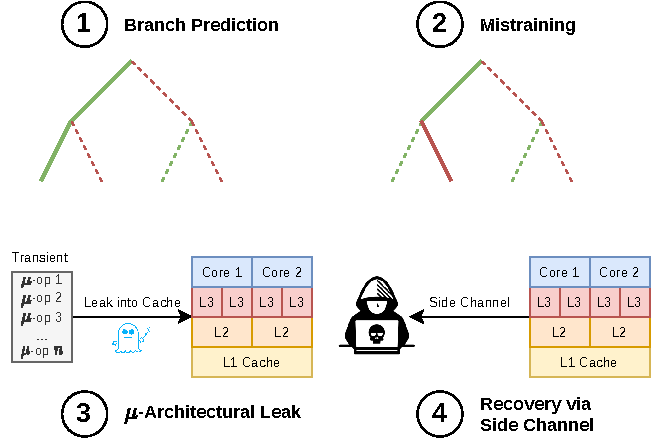
\includegraphics[width=0.8\linewidth]{figs/overview.pdf}
  \end{column}
\end{columns}
\end{frame}
\endgroup

\begin{frame}[c]{Goals}
  \begin{enumerate}
    \item Provide an overview of Spectre attacks
    \vfill
    \item Differentiate Spectre from Meltdown (variant 3)
    \vfill
    \item Present proof of concept exploits for Spectre variant 1 and 2
    \vfill
    \item Evaluate the practical risks associated with Spectre attacks
    \vfill
    \item Present future avenues for Spectre exploitation (variant 4, other side channels)
    \vfill
    \item Discuss and propose mitigations against current/future Spectre attacks
  \end{enumerate}
\end{frame}

\begin{frame}[c]{Threat Model and Assumptions}{}
  {\bf Overview:}
  \begin{itemize}
    \item Strong threat model, limited assumptions about attacker's capabilities
    \item Roughly similar threat model to the Meltdown paper
  \end{itemize}

  \vfill
  {\bf Attacker Capabilities:}
  \begin{itemize}
    \item Attacker can spawn a process in user mode with {\bf ordinary user-level privileges}
    \item Ability to pass parameters to the victim
    \begin{itemize}
      \item E.g.~RPC, system calls, sockets, file I/O, library calls, etc.
    \end{itemize}
    \item For attacks against KVM, we assume ring 0 access in the {\bf guest OS only}
  \end{itemize}

  \vfill
  {\bf Other Assumptions:}
  \begin{itemize}
    \item Processor that supports speculative execution
    \begin{itemize}
      \item Before $\mu$-architectural updates circa 2019
      \item Dynamic branch prediction (trainable)
    \end{itemize}
    \item Some shared memory between attacker and victim (if another process)
    \begin{itemize}
      \item E.g.~a shared library mapped to same physical memory
    \end{itemize}
  \end{itemize}
\end{frame}

%\begin{frame}[c]{Relevance and Impact}
%  \begin{itemize}
%    \item Foo
%  \end{itemize}
%\end{frame}

\begingroup
\setwatermark{}
\begin{frame}[c]{Spectre vs Meltdown (tl;dr)}
  \begin{columns}
    \begin{column}[t]{0.5\textwidth}
      \centering
      \includesvg[height=6em]{figs/logos/meltdown.svg}
      \begin{itemize}
        \item Dumps arbitrary kernel memory
        \begin{itemize}
          \item And thus physical memory
        \end{itemize}
        \item Victim is mapped kernel memory
        \begin{itemize}
          \item No victim process required
        \end{itemize}
        \item Mostly stopped by KPTI (KAISER) mitigation
        \item Affects only some CPUs (mostly Intel)
        \item Easier to exploit, easier to mitigate
      \end{itemize}
    \end{column}

    \begin{column}[t]{0.5\textwidth}
      \centering
      
\includegraphics[height=6em]{figs/logos/spectre.png}
      \begin{itemize}
        \item Leaks secrets via speculative execution
        \item Victim is another process or the kernel
        \begin{itemize}
          \item But can also be the same process
        \end{itemize}
        \item Totally unaffected by KPTI
        \item Affects a wide range of CPUs
        \begin{itemize}
          \item Multiple vendors
        \end{itemize}
        \item Harder to exploit, harder to mitigate
      \end{itemize}
    \end{column}
  \end{columns}
\end{frame}
\endgroup

\begin{frame}[c]{Spectre Building Blocks}
  \begin{enumerate}
    \item {\bf\color{blue}Setup Phase}
    \begin{itemize}
      \item Mistrain the CPU's branch predictor
      \item Optionally: Induce speculative execution (e.g.~evict branch-specific value $n$ from the cache)
    \end{itemize}

    \vfill
    \item {\bf\color{orange}Execution Phase}
    \begin{itemize}
      %\item Attacker provides some attacker-controlled value to victim (e.g.~$n = 3000000$)
      %\begin{itemize}
      %  \item Could be via a system call, a socket, file I/O, etc.
      %  \item Or the victim could be our own process (much simpler)
      %\end{itemize}
      \item CPU mispredicts a branch on the value of $n$
      \begin{itemize}
        \item In variant 1, this is provided by the attacker (e.g.~via system call, socket, file I/O, RPC, etc.)
        \item We'll touch on variant 2 later
      \end{itemize}
      \item CPU speculatively executes the incorrect branch
      \item Transient instructions encode a secret value $v$ (dependent on $n$) into $\mu$-architectural state
    \end{itemize}

    \vfill
    \item {\bf\color{green}Recovery Phase}
    \begin{itemize}
      \item Attacker recovers information about $v$ using a $\mu$-architectural side channel
      \item E.g.~flush+reload, evict+reload, evict+time
    \end{itemize}
  \end{enumerate}
\end{frame}

\begin{frame}[c]{Branch Prediction}
  \begin{itemize}
    \item Code branches depend on value(s) in memory
    \begin{itemize}
      \item \code{if (foo < size) \{ A(foo); \} else \{ B(foo); \}}
      \item Which path we take depends on \code{foo} and \code{size}
    \end{itemize}

    \vfill
    \item But fetching these values can be slow
    \begin{itemize}
      \item Suppose that foo is a cache hit but size is a cache miss
      \item If CPU is idle during this time, we lose out on performance
      \item Wasting clock cycles
    \end{itemize}

    \vfill
    \item So what can the CPU do?
    \begin{itemize}
      \item Make a guess and just roll with it while fetching the value
      \item If our guess is right, great! We saved some time
      \item Otherwise, roll back (\textit{retire}) erroneous state changes and execute correct code
    \end{itemize}
  \end{itemize}
\end{frame}

\fullframegraphic{figs/silly/this_is_fine.jpg}

\begin{frame}[c]{But There is One Small (Huge) Problem}{}
  {\bf Transient Instructions}
  \begin{itemize}
    \item Incorrect branch predictions are retired
    \item But $\mu$-architectural effects remain
    \item Number of transient instructions depends on the size of the CPU's reorder buffer
    \item Can be quite high in practice (in some CPUs 192 $\mu$-ops $\sim$ 180ish ops)
  \end{itemize}

  \vfill
  {\bf Why is This a Problem?}
  \begin{itemize}
    \item Erroneous effects are encoded in $\mu$-architectural state, e.g.~cache memory
    \item This \textit{should} be totally transparent to the architectural state
    \item But attackers can transfer $\mu$-architectural state into architectural state via side channels
  \end{itemize}
  %\begin{itemize}
  %  \item An incorrect branch prediction leads to \alert{transient instructions}
  %  \begin{itemize}
  %    \item (c.f.~Meltdown from last week)
  %  \end{itemize}

  %  \vfill
  %  \item Ordinarily rolled back (\alert{retired}) by the CPU

  %  \vfill
  %  \item But these transient instructions have \alert{micro-architectural side effects}
  %  \begin{itemize}
  %    \item From the architecture's perspective, effects are rolled back
  %    \item But the \alert{cache remains affected}
  %  \end{itemize}
  %\end{itemize}
\end{frame}

\begingroup
\setwatermark{}
\begin{frame}[c]{Branch Prediction Illustrated}
  \begin{center}
    \color{black}
    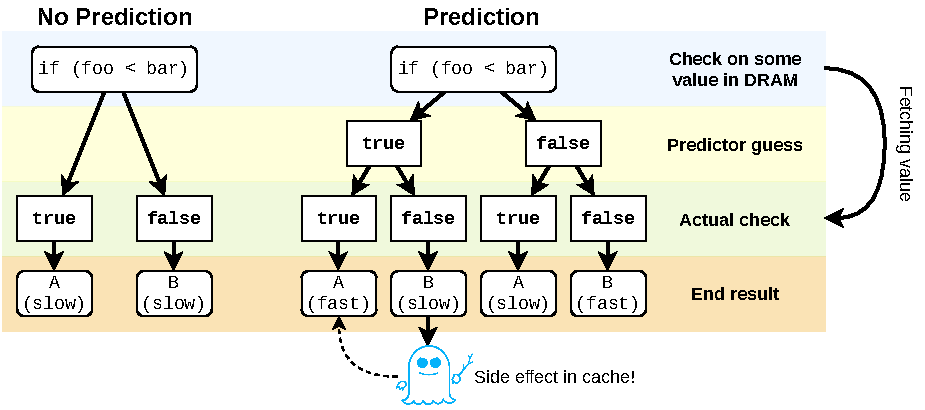
\includegraphics[width=0.9\textwidth]{figs/prediction.pdf}
  \end{center}
\end{frame}
\endgroup

\begin{frame}[c]{(Mis)Training the Branch Predictor}{}
  {\bf How to Induce Speculative Execution?}
  \begin{itemize}
    \item Dynamic branch predictors\footnote{Mittal \cite{mittal2019_branch_prediction} is a nice resource for those who want an in-depth study of branch prediction techniques} update their prediction model using historical data
    \item The attacker can invoke a specific branch target
    \begin{itemize}
      \item E.g.~Use a \code{foo} such that \code{foo < size}
      \item Number of times they need to do this depends on BP implementation
    \end{itemize}
  \end{itemize}

  \vfill
  {\bf After Mistraining}
  \begin{itemize}
    \item Attacker can supply an out-of-bounds \code{foo}
    \begin{itemize}
      \item But the branch predictor will still execute as if \code{foo < size}
      \item Transient code accesses some secret at an offset computed using \code{foo}
      \item That secret leaks into cache memory
    \end{itemize}
  \end{itemize}
\end{frame}

\begin{frame}[c]{Transferring Leaked Data into Architectural State}
  \begin{itemize}
    \item $\mu$-architectural side channels can transfer leaked information into architectural state
    \item The Spectre paper primarily focuses on cache-based side channels
    \begin{itemize}
      \item But in principle \textit{any} observable effects can leak information
      \item E.g.~contention for execution units or traditional side channels such as power draw
    \end{itemize}
  \end{itemize}

  \vfill
  {\bf Flush+Reload}
  \begin{itemize}
    \item Flush a cache line via {\tt clflush} and time subsequent access (low time $\rightarrow$ cache hit $\rightarrow$ victim has accessed)
  \end{itemize}

  \vfill
  {\bf Evict+Reload}
  \begin{itemize}
    \item Similar to Flush+Reload but we evict the cache via contention instead (works without {\tt clflush})
  \end{itemize}

  \vfill
  {\bf Evict+Time}
  \begin{itemize}
    \item Rather than directly reloading, we time an operation that depends on the state of the cache
  \end{itemize}
\end{frame}

\begin{frame}[c,fragile]{Direct and Indirect Branching}
  \begin{columns}
    \begin{column}[t]{0.5\textwidth}
      {\bf\color{blue}\Large Direct Branches}
      \begin{itemize}
        \item Conditionals, switches, ternary operators, etc.
        \item Prediction may not match real check
      \end{itemize}

      \vspace{1em}
      \begin{listing}[language=c,gobble=8,xleftmargin=5em]
        const size_t size = 256;
        int arr[size];

        void my_fn(int foo) {
            if (foo < size) {
                /* Do something with arr and foo */
            }
        }
      \end{listing}
    \end{column}

    \begin{column}[t]{0.5\textwidth}
      {\bf\color{orange}\Large Indirect Branches}
      \begin{itemize}
        \item Call based on function pointer (address)
        \item Predictor can guess an incorrect address
      \end{itemize}

      \vspace{1em}
      \begin{listing}[language=c,gobble=8,xleftmargin=5em]
        int my_fn(int foo) {
            return foo * foo;
        }

        /* ... */

        int (*fn_ptr)(int) = &my_fn;
        fn_ptr(42);
      \end{listing}
      %{\footnotesize Results in:}
      %\begin{listing}[language=x64,gobble=8]
      %  ; ...
      %  leaq	my_fn(%rip), %rax
      %  movq	%rax, -8(%rbp)
      %  movq	-8(%rbp), %rax
      %  movl	$42, %edi
      %  call	*%rax
      %  ; ...
      %\end{listing}
    \end{column}
  \end{columns}
\end{frame}

\begin{frame}[c]{Spectre Variants}{}
  {\bf Variant 1: Conditional Branch Misprediction}
  \begin{itemize}
    \item Abuses speculation in {\bf\color{blue}Direct Branches}
    \item Attacker tricks CPU into executing the wrong branch of a conditional
  \end{itemize}

  \vfill
  {\bf Variant 2: Indirect Branch Poisoning}
  \begin{itemize}
    \item Abuses speculation in {\bf\color{orange}Indirect Branches}
    \item Attacker tricks CPU into invoking a {\bf Spectre gadget} instead of following a legit function pointer
  \end{itemize}

  \vfill
  {\bf Variant 4: Speculative Store Bypass (Spectre-NG)}
  \begin{itemize}
    \item Abuses speculation in CPU's {\bf\color{green}Store-To-Load} forwarding logic
    \item We will cover this if we have time
  \end{itemize}
\end{frame}

\begin{frame}[c, fragile]{Variant 1: Conditional Branch Misprediction}
  \begin{columns}
    \begin{column}[t]{0.35\textwidth}
      {\bf Basic Idea}
      \begin{itemize}
        \item Trick CPU into performing out of bounds access
        \item Encode secret into cache memory
        \item Transfer using a side channel
      \end{itemize}

      \vspace{0.5em}
      {\bf Toy Example}
      \begin{listing}[language=c,gobble=8,xleftmargin=1em]
        const size_t arr1_size = 16;
        int arr1[16];
        int arr2[256 * 512];

        void victim(int foo) {
            if (foo < arr1_size) {
                int x = arr2[arr1[foo] * 512];
            }
        }
      \end{listing}
    \end{column}

    \begin{column}[t]{0.65\textwidth}
      {\bf Steps in the Attack}
      \begin{enumerate}
        \item Flush or evict \code{arr2} from the cache.
        \item Train CPU by repeatedly calling \code{victim(0)} or similar.
        \begin{itemize}
          \item CPU now thinks the \code{if}-statement will be \code{true}
        \end{itemize}
        \item Choose some \code{malicious = \&secret - arr}.
        \begin{itemize}
          \item Thus \code{arr + malicious == &secret} \\
                and \code{arr[malicious] == secret}
        \end{itemize}
        \item Flush or evict \code{arr1\_size} to induce speculative execution.
        \item Invoke \code{victim(malicious)}.
        \item Probe each entry in \code{arr2} and time access.
        \begin{itemize}
          \item Fast access $\rightarrow$ cache hit $\rightarrow$ 1
          \item Slow access $\rightarrow$ cache miss $\rightarrow$ 0 or error
        \end{itemize}
      \end{enumerate}
    \end{column}
  \end{columns}
  \ufootnote{Toy example is based on the Spectre paper \cite{kocher2019_spectre}.}
\end{frame}

\begin{frame}[c]{Variant 1 Examples}{}
  {\bf Attack on V8 JavaScript Engine}
  \begin{itemize}
    \item Browsers rely on strong isolation between untrusted JavaScript and the rest of the browser
    \begin{itemize}
      \item E.g.~JavaScript on one page shouldn't be able to mess with another page
    \end{itemize}
    \item Spectre can totally break this isolation
    \item Malicious JavaScript code is only a few lines long, can leak arbitrary browser data
    \begin{itemize}
      \item Requires a high resolution timer implementation (via web workers)
      \item No {\tt clflush} instruction, requires an eviction strategy instead
    \end{itemize}
  \end{itemize}

  \vfill
  {\bf Attack on eBPF}
  \begin{itemize}
    \item eBPF subsystem is design to allow userspace to make safe extensions to the kernel
    \begin{itemize}
      \item Primary use case is observability
      \item Safety is enforced by a verifier, including safe memory access
      \item Spectre totally breaks these safety guarantees
    \end{itemize}
    \item Attack targets eBPF map data structures
    \begin{itemize}
      \item Trick the CPU into accessing arbitrary user memory instead of map entries
      \item PoC requires a CPU without SMAP, but it's possible to work around this
    \end{itemize}
  \end{itemize}
\end{frame}

\begin{frame}[c,fragile]{Variant 1 Examples (Not in the Paper)}{}
  {\bf Linux Kernel {\tt swapgs} Bypass}
  \begin{itemize}
    \item CPU provides a special instruction {\tt swapgs} which the kernel calls on interrupt or exception
    \item An attacker can speculatively bypass a {\tt swapgs} check in the kernel
    \item This would allow them to access arbitrary percpu kernel memory
    \begin{itemize}
      \item Would still need to transfer using cache side channels though
    \end{itemize}
  \end{itemize}

  \vfill
  The attacker would bypass the following check:
  \begin{listing}[language=c,gobble=4,xleftmargin=1em]
    if (/* Coming from user space */)
      asm volatile ("swapgs");
    /* Business logic down here, reading percpu values
     * Gets speculatively executed without swapgs */
  \end{listing}

  \vfill
  \begin{listing}[language=none,gobble=4,xleftmargin=1em]
    lscpu:
    Vulnerability Spectre v1:        Mitigation; usercopy/swapgs barriers and __user pointer sanitization
  \end{listing}

  \ufootnote{Based on Linux kernel docs \cite{linux_hwvuln}.}
\end{frame}

\begin{frame}[c, fragile]{Mitigating Variant 1}{Index Masking}
  \begin{itemize}
    \item Mask indices such that they are strictly bounded by array size
    \item Steers array accesses into safe memory regions
    \item JITed or interpreted code can do this automatically
    \begin{itemize}
      \item E.g.~The eBPF runtime now injects masking logic before all array accesses
      \item This is possible with the help of the verifier, which enforces bounds checking
    \end{itemize}
  \end{itemize}

  \vfill
  How it works in eBPF:\\
  \hspace{6em}
  \begin{minipage}{8em}
    \begin{listing}[language=c,gobble=6]
      if (i < 256) {
          x = arr[i];
      }
    \end{listing}
  \end{minipage}
  $\xRightarrow{\text{Becomes}}$
  \hspace{2em}
  \begin{minipage}{12em}
    \begin{listing}[language=c,gobble=6]
      if (i < 256) {
          x &= ~(long)(i | (256 - 1 - i)) >> 63;
          x = arr[i];
      }
    \end{listing}
  \end{minipage}

  \vfill
  \begin{itemize}
    \item If $0 \le x < 256$, we get mask = \texttt{0xffffffffffffffff}
    \begin{itemize}
      \item And thus \code{i & mask == i}
    \end{itemize}
    \item If $x < 0$ or $x \ge 256$, we get mask = \texttt{0x0}
    \begin{itemize}
      \item And thus \code{i & mask == 0}
    \end{itemize}
  \end{itemize}
\end{frame}

\begin{frame}[c, fragile]{Mitigating Variant 1}{Index Masking}
  \begin{columns}
    \begin{column}{0.5\textwidth}
      {\bf Before Index Masking}
      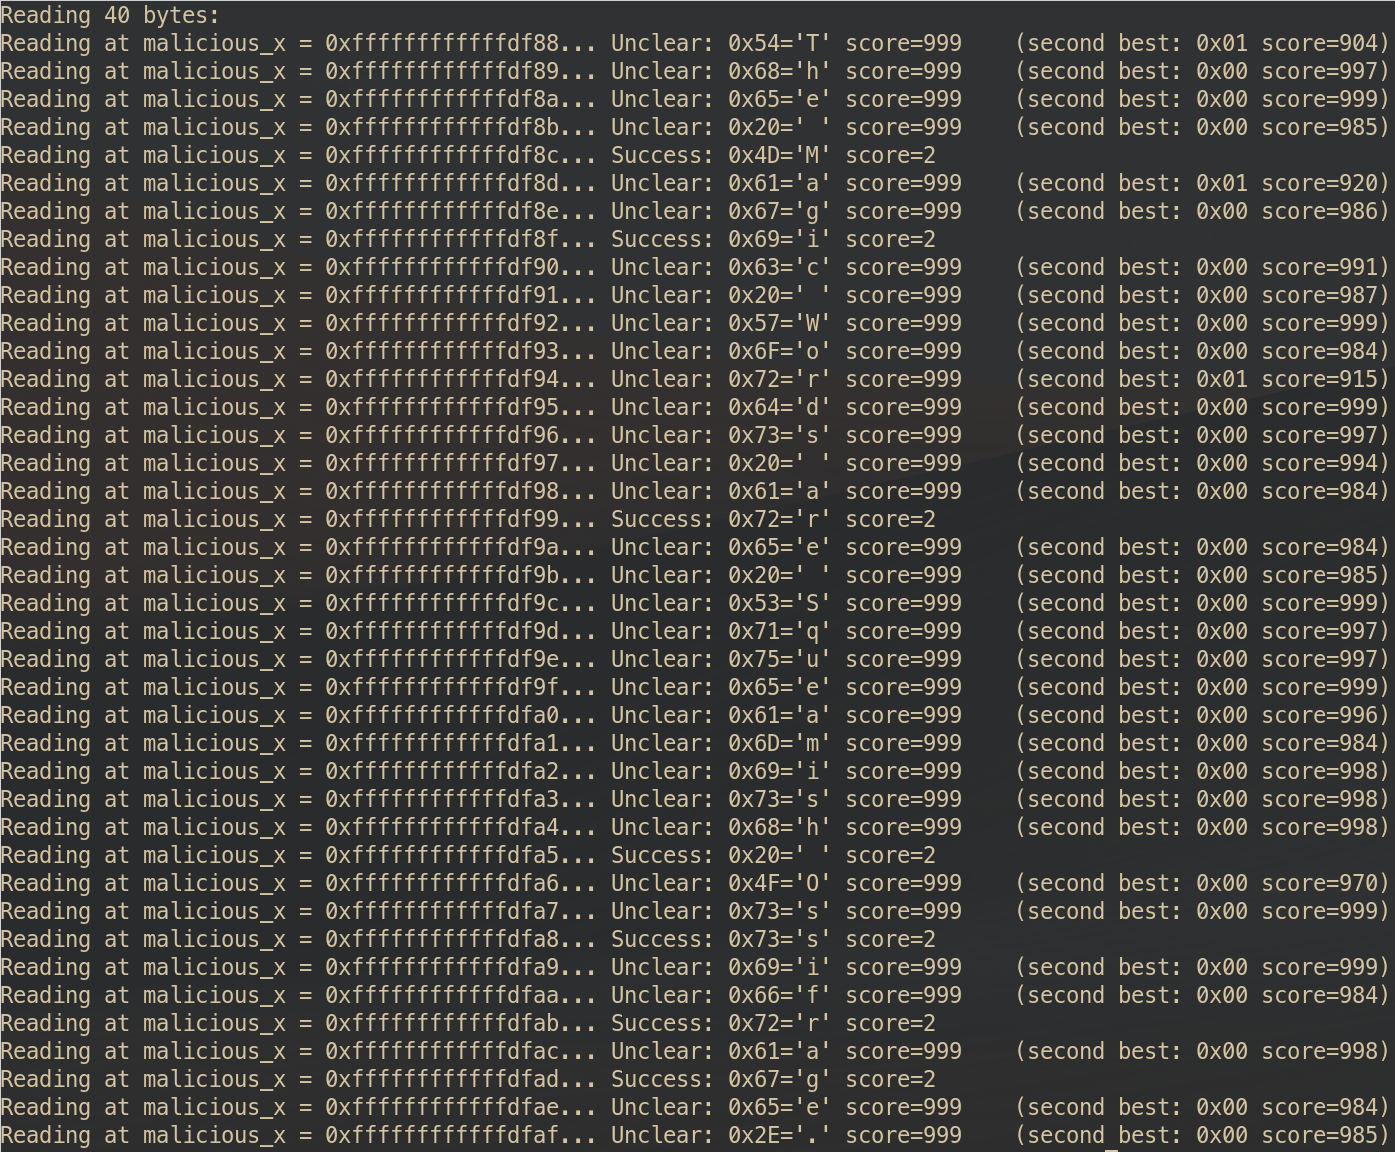
\includegraphics[width=\columnwidth]{figs/screenshots/poc.png}
    \end{column}
    \begin{column}{0.5\textwidth}
      {\bf After Index Masking}
      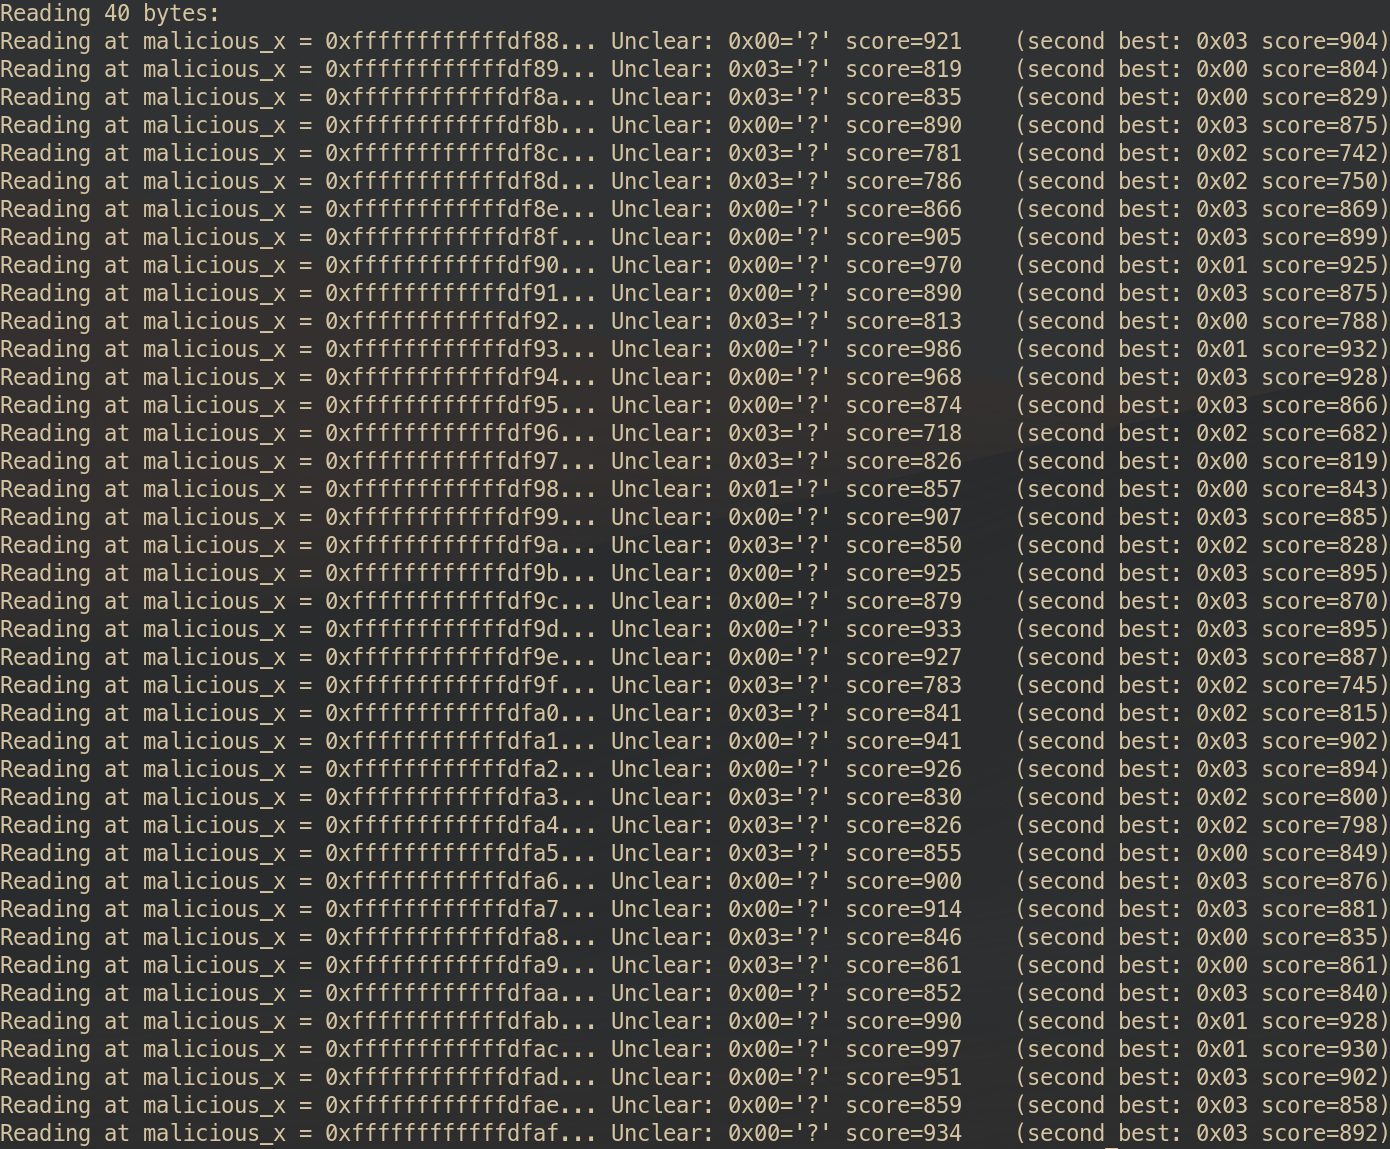
\includegraphics[width=\columnwidth]{figs/screenshots/poc_patched.png}
    \end{column}
  \end{columns}
\end{frame}

\begin{frame}[c]{Mitigating Variant 1}{Poison Pointers}
  {\bf Overview}
  \begin{itemize}
    \item The idea is to make pointers unusable unless you have some pseudo-random value $x$
    \item Simply XOR all pointers $p$ by some $x$
    \item At runtime, decode $p$ by repeating same XOR operation
  \end{itemize}

  \vfill
  {\bf End Result}
  \begin{itemize}
    \item Adversary who does not know a poison value cannot use a pointer
    \item But it's still possible to leak the poison value via side channel
    \item This probably works best in combination with other defences
  \end{itemize}
\end{frame}

\begin{frame}[c, fragile]{Variant 1: Evaluation}{}
  {\bf Requirements}
  \begin{itemize}
    \item Generally requires either:
      \begin{enumerate}
        \item Attacker is in the same process as the victim (e.g.~web browser)
        \item Some shared memory + ability to pass parameters to victim (e.g.~RPC, system calls, file I/O)
      \end{enumerate}
    \item While requirements are \textit{slightly} limiting, there are {\bf a ton} of real-world scenarios\\
    where variant 1 is problematic
    \begin{itemize}
      \item We have seen this from the examples
      \item eBPF + JavaScript are \textit{widely} used
      \item Crypto libraries? Almost certainly affected
    \end{itemize}
  \end{itemize}

  \vfill
  {\bf Ease of Mitigation}
  \begin{itemize}
    \item JITed and interpreted languages have an easier time mitigating variant 1
    \begin{itemize}
      \item eBPF, V8 JavaScript, Python, etc.
    \end{itemize}
    \item But legacy applications are still vulnerable, not strictly trivial to update
    \item Can use static analysis techniques to identify possible variant 1 vulnerabilities
  \end{itemize}
\end{frame}

\begin{frame}[c, fragile]{Variant 1: Evaluation}{}
  {\bf Speed of the Attack}
  \begin{itemize}
    \item Toy example can do 10KB/s
    \item eBPF attack is on the order of 2KB/s to 5KB/s
    \item JavaScript attack speed is not presented, but we can expect this to be much lower
    \begin{itemize}
      \item Lack of a native high resolution timer
      \item Must rely on eviction rather than flushing
    \end{itemize}
    \item Speed is not great, but acceptable, especially if attacker can amortize over a rough estimation of secret location
  \end{itemize}

  \vfill
  {\bf Accuracy of Recovered Data}
  \begin{itemize}
    \item Similar accuracy issues to Meltdown
    \item Limited accuracy of timing measurements + unexpected caching / eviction
    \item Can achieve low error rates, especially with multiple iterations
    \begin{itemize}
      \item Repetition-only: $\sim0.005\%$
    \end{itemize}
  \end{itemize}
\end{frame}

\begin{frame}[c,fragile]{Variant 2: Indirect Branch Poisoning}{}
  {\bf Overview}
  \begin{itemize}
    \item This attack relies on tricking the CPU into executing a {\bf Spectre gadget} in an indirect branch
    \begin{itemize}
      \item Recall: Indirect branches result from function pointers
    \end{itemize}
    \item The CPU keeps track of visited indirect branches in the {\bf BTB} (Branch Target Buffer)
    \begin{itemize}
      \item Details vary depending on the CPU (number of prior addresses, which address bits are tracked)
    \end{itemize}
    \item We need to train the CPU's BTB to point to our chosen gadget
    \begin{itemize}
      \item Training involves mimicking victim's access patterns, then making a jump to the chosen address
    \end{itemize}
  \end{itemize}

  \vfill
  {\bf Spectre Gadget}
  \begin{itemize}
    \item Similar to ROP, the attacker locates a \textit{gadget} which performs some desirable operation
    \item In practice, these gadgets can be quite simple
    \item Training is as simple as invoking the function pointer after setting it to our gadget address
    \begin{itemize}
      \item The gadget doesn't even need to exist in our own process! Just needs to be same address
    \end{itemize}
  \end{itemize}
\end{frame}

\begingroup
\setwatermark{}
\begin{frame}[c]{Variant 2: Indirect Branch Poisoning}{}
  \begin{columns}
    \begin{column}{0.5\textwidth}
      {\bf So the Steps Are\ldots}
      \begin{enumerate}
        \item Identify a Spectre gadget.
        \item Find it in victim memory.
        \item Train CPU to speculatively execute that location.
        \item Induce speculative execution.
        \item Transfer leaked data via side channel.
      \end{enumerate}
    \end{column}

    \begin{column}{0.5\textwidth}
      \color{black}%
      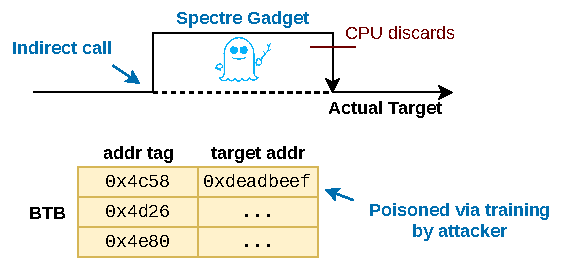
\includegraphics[width=1\columnwidth]{figs/indirect.pdf}%
    \end{column}
  \end{columns}

  \ufootnote{Figure based on information in Intel whitepaper \cite{intel_retpoline}.}
\end{frame}
\endgroup

\begin{frame}[c]{Variant 2 Examples}{}
  {\bf PoC on a Windows DLL}
  \begin{itemize}
    \item Static analysis techniques on {\tt nttdll.dll} to identify a Spectre gadget
    \item That gadget can read victim memory with an attacker-controlled \texttt{edx} and \texttt{edi}
    \begin{itemize}
      \item Set {\tt edx} to the base address of a probe array
      \item Set {\tt edi} to a target address minus some offset
    \end{itemize}
    \item Training the BTB is accomplished by repeatedly invoking a modified version of {\tt Sleep()} in the attacker's own address space
    \item ASLR is insufficient to protect the victim---only a few iterations need to be done to identify the correct training sequence
    \item It's not hard to imagine that similar attacks are possible on crypto libraries, etc.
  \end{itemize}
\end{frame}

\begin{frame}[c]{Variant 2 Examples}{}
  {\bf Defeating KVM Isolation}
  \begin{itemize}
    \item Requires attacker to having ring 0 access in the guest OS
    \begin{itemize}
      \item This presents practical limitations for KVM attacks in the cloud for example
    \end{itemize}
    \item Find hypervisor ASLR offset by analyzing Branch Target Buffer and Branch History Buffer leaks
    \item Use a Spectre gadget to find cache set information + location of physical memory map
    \item Execute another gadget found in the eBPF interpreter
    \begin{itemize}
      \item Use this gadget to dump arbitrary host memory
    \end{itemize}
  \end{itemize}
\end{frame}

\begin{frame}[c]{Mitigating Variant 2}{Extensions to the ISA}
  {\bf Indirect Branch Restricted Speculation (IBRS)}
  \begin{itemize}
    \item Prevents unprivileged indirect branches from affecting privileged branch predictions
    \item Processor enters a special IBRS mode
    \item Ignores any changes made outside IBRS mode
  \end{itemize}

  \vfill
  {\bf Single Thread Indirect Branch Prediction (STIBP)}
  \begin{itemize}
    \item Prevent hyperthreaded software running in same core from sharing branch predictions
    \item Indirect branch predictors are never shared across cores \cite{intel_stibp}
    \item So this would prevent two processes running in same core from influencing each other
  \end{itemize}
\end{frame}

\begin{frame}[c]{Mitigating Variant 2}{Extensions to the ISA}
  {\bf Indirect Branch Predictor Barrier (IBPB)}
  \begin{itemize}
    \item Provides a barrier that works like IBRS
    \item Software running before the barrier cannot affect branch prediction after the barrier
  \end{itemize}

  \vfill
  {\bf Applying the Update}
  \begin{itemize}
    \item Extensions are applied via a microcode update
    \item Requires BIOS and OS support
    \item Overhead varies depending on how the mitigations are deployed / used
    \begin{itemize}
      \item Restricting mitigations to kernelspace and selected shared libraries might be sufficient, depending on use case
      \item Deploying mitigations system-wide can incur significant overhead
    \end{itemize}
  \end{itemize}
\end{frame}

\begingroup
\setwatermark{}
\begin{frame}[c,fragile]{Mitigating Variant 2}{Retpolines}
  \begin{columns}
    \begin{column}[t]{0.5\textwidth}
      \begin{itemize}
        \item Retpolines work by replacing indirect calls with a return-based trampoline
        \item Works as follows:
        \begin{enumerate}
          \item Push the function address onto the stack
          \item Replace the indirect call with a jump into a dummy loop
          \item Gate the start of the loop with {\tt lfence} and {\tt pause} to prevent speculation and spin forever
          \item Call {\tt ret} to jump into the correct function
        \end{enumerate}
        \item This can be applied automatically at compile time (gated by a compiler flag)
        \item The Linux kernel now compiles with this by default
      \end{itemize}
    \end{column}

    \begin{column}[t]{0.5\textwidth}
      \begin{listing}[language=x64,gobble=8,xleftmargin=6em]
        __x86_indirect_thunk_rax:
        .LFB2:
          call	.LIND1
        .LIND0:
          pause
          lfence
          jmp	.LIND0
        .LIND1:
          mov	%rax, (%rsp)
          ret
      \end{listing}
      \vspace{1em}
      \color{black}%
      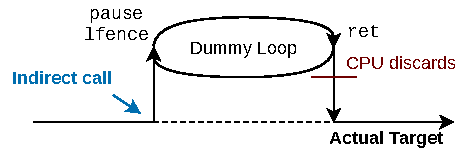
\includegraphics[width=0.9\columnwidth]{figs/retpoline.pdf}%
    \end{column}
  \end{columns}

  \ufootnote{Figure based on information in Intel whitepaper \cite{intel_retpoline}.}
\end{frame}
\endgroup

\begin{frame}[c, fragile]{Variant 2: Evaluation}{}
  {\bf Requirements}
  \begin{itemize}
    \item Attacker needs to find one or more Spectre gadgets to achieve their goal
    \begin{itemize}
      \item Requires static analysis or similar techniques
    \end{itemize}
    \item Need to defeat ASLR to figure out the correct training sequence
    \begin{itemize}
      \item In practice this requires a guess and check strategy
    \end{itemize}
    \item For KVM bypass, attacker requires access to ring 0 in the guest OS
    \begin{itemize}
      \item This may be unrealistic in cloud contexts (i.e.~containers running in VMs)
    \end{itemize}
  \end{itemize}

  \vfill
  {\bf Ease of Mitigation}
  \begin{itemize}
    \item Mitigations can be applied automatically
    \item But applying them everywhere can incur significant performance overhead
    \item Defenders need to consider carefully what code they want to protect
  \end{itemize}
\end{frame}

\begin{frame}[c, fragile]{Variant 2: Evaluation}{}
  {\bf Speed of the Attack}
  \begin{itemize}
    \item Setup phase can be incredibly slow
    \item KVM attack takes 20--30 minutes for initial setup phase
    \item In general, data transfer rate is \textit{insanely slow}
    \begin{itemize}
      \item Only 41B/s for Windows DLL attack and 1.8KB/s for KVM attack
      \item Could be due to difficulty training (and re-training) the BTB + complexity of combining gadgets
      \item Could also be due to higher error rates
    \end{itemize}
  \end{itemize}

  \vfill
  {\bf Accuracy of Recovered Data}
  \begin{itemize}
    \item Higher error rates in variant 2 than in variant 1
    \item About 2\% error rate for Windows DLL attack and 1.7\% for KVM attack
    \item We can expect similar attacks to have about equivalent error rate
  \end{itemize}
\end{frame}

\begin{frame}[c]{Other Mitigation Strategies}{}
  {\bf Limiting Availability of High Resolution Timers}
  \begin{itemize}
    \item Limit the resolution of available timers + introduce some jittering
    \item Doesn't directly stop the attack, only raises the error rate
    \item Also wouldn't work for lower-level languages---high resolution timers are critical for many applications
  \end{itemize}

  \vfill
  {\bf Mitigating Side Channels Directly}
  \begin{itemize}
    \item Other direct mitigations could be applied to limit side channels
    \item E.g.~future processors can track potentially secret data and prevent leaks into cache state
    \item Would be quite difficult to mitigate every single side channel
  \end{itemize}

  \vfill
  {\bf Disabling Speculative Execution}
  \begin{itemize}
    \item System-wide, this is almost definitely not the right approach
    \item Would introduce a huge performance hit (but might be appropriate for specific applications, e.g.~via {\tt lfence})
  \end{itemize}
\end{frame}

\begin{frame}[c]{Anomaly Detection?}{}
  \begin{itemize}
    \item Anomaly detection is something I've been thinking about as an indirect mitigation strategy
    \begin{itemize}
      \item Not really in the spirit of trusted computing
      \item But it's something I'm quite interested in
    \end{itemize}

    \vfill
    \item My observation: Spectre-style attacks almost always involve {\bf repeated weird behaviour}
    \begin{itemize}
      \item Anomaly detection is {\it really good\/} at flagging {\bf repeated weird behaviour}
      \item Catch the attackers in the act, possibly kill the processes they are using for training
    \end{itemize}

    \vfill
    \item As far as I know, nobody has investigated anomaly detection vs Spectre
    \begin{itemize}
      \item Would be interesting to see how effective it can be as a stop-gap mitigation
      \item There would also be something very poetic about an eBPF-based IDS stopping Spectre in its tracks
    \end{itemize}
  \end{itemize}
\end{frame}

\begin{frame}[c]{Discussion Questions}
  \begin{enumerate}
    \item How can we help prevent something like Spectre and Meltdown from happening in the future?
    \begin{itemize}
      \item Move towards an open CPU design (e.g.~something similar to RISC-V)?
      \item Introduce regulations mandating independent audits of ISA design?
    \end{itemize}

    \vfill
    \item Is Spectre something you think you should be practically worried about (e.g.~attackers potentially exploiting Spectre on your personal computer)? Why or why not?

    \vfill
    \item Spectre mitigations can introduce moderate to severe performance penalties depending on how widely they are deployed. What do you think would define a reasonable protection boundary for applying mitigations?
    \begin{itemize}
      \item Kernel only?
      \item Kernel plus some userspace applications/libraries?
      \item Every single piece of software on the system?
    \end{itemize}
  \end{enumerate}
\end{frame}

\appendix

\section{Backup Slides}

\section{References}

\nocite{*}
\begin{frame}[allowframebreaks, noframenumbering, plain]
  \frametitle{References}
  \sloppy
  \printbibliography
\end{frame}

\end{document}

% vim:syn=tex

